\documentclass{article}
\usepackage{graphicx}% Required for inserting images
\usepackage{lindrew}
\usepackage[shortlabels]{enumitem}
\usepackage{enumerate}
\usepackage{algorithm}
\usepackage{algpseudocode}
\usepackage{pythonhighlight}

\title{CS 156a Problem Set 2}
\author{Amitesh Anand Pandey}
\date{October 2024}

\begin{document}
\maketitle
\section*{Hoeffding Inequality}
\subsection*{Problem 1}
\begin{figure}[htp]
    \centering
    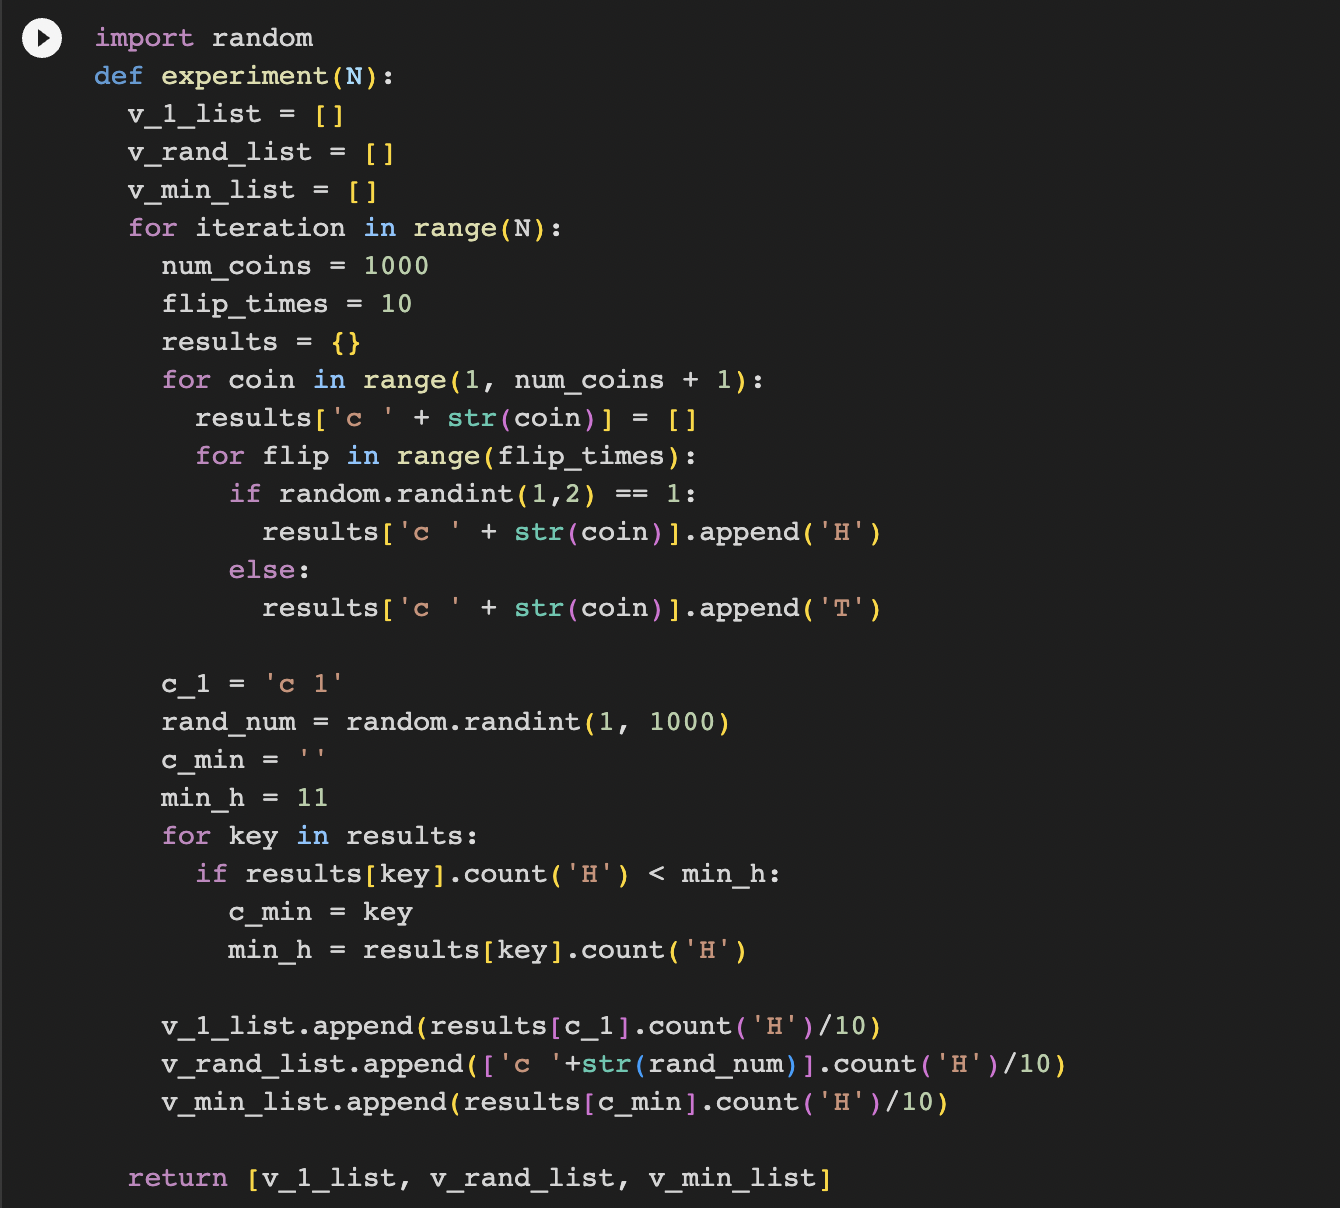
\includegraphics[width=4in]{Screen Shot 2023-07-04 at 8.19.46 PM.png}
    \caption{Experiment Code}
    \label{fig:galaxy}
\end{figure}
\begin{figure}[htp]
    \centering
    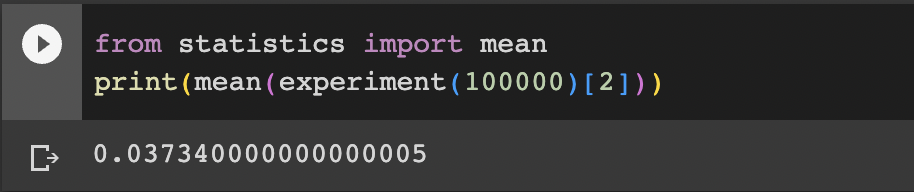
\includegraphics[width=4in]{Screen Shot 2023-07-04 at 8.19.33 PM.png}
    \caption{Result after 100000 simulations}
    \label{fig:galaxy}
\end{figure}
Thus, the correct option is \textbf{[b]}.
\newpage
\subsection*{Problem 2}
For the first coin $c_{1}$, the distribution of $\nu_{1}$ would closely model $\mu$ since it is a fair coin with no apriori bias introduced. Similarly with $c_{\text{rand}}$, although it is not the same coin's outcomes each time, it is identical to the first case in that each of those 100000 sequence of flips were picked at random from all possible sequences. Thus $\nu_{\text{rand}}$ would also closely model $\mu$. However, with $\nu_{\text{min}}$, only a very special type of coin is considered in each of the simulations, this cannot be expected to resemble a fair coin in its outcomes. Thus the correct option is $\textbf{[d]}$, $c_{1} \text{ and }c_{\text{rand}}$. 
\section*{Error and Noise}
\subsection*{Problem 3}
Note that there are two situations in which $h$ incorrectly approximates $f$, these are given by $h(x) \neq f(x) = y$, and $h(x) = f(x) \neq y$. The first situation has probability $\mu \lambda$ and the second has probability $(1-\mu)(1-\lambda)$. We discard the case of $h(x) \neq f(x) \neq y$ because the ones are introduce error are contained in the previous two cases. When adding probabilities, we must make sure that the events we are adding up are disjoint. The probability finally is $(1-\mu)(1-\lambda) + \mu \lambda$ or option $\textbf{[e]}$. 
\subsection*{Problem 4}
Expanding the solution to the previous problem, we get that $h$ approximates $y$ with error $1 - \mu - \lambda + 2\lambda\mu$. This makes it clear that we want $\mu = 2\lambda\mu$ for the $\mu$ terms to cancel out. This occurs at $\lambda = 0.5$, thus the correct option is $\textbf{[b]}$. 
\section*{Linear Regression}
\subsection*{Problem 5}
Using linear regression and setting the number of experiments to 1000, the mean $E_{\text{in}}$ I obtained was $\approx 0.04$, which means it was closest to $0.1$, so the correct option is $\textbf{[c]}$. 
\subsection*{Problem 6}
Generating a 1000 out of sample points, and calculating $E_{\text{out}}$ over these as out of sample error for a 1000 hypotheses (different $g$'s), I obtained $E_{\text{out}} \approx 0.045$, which means, it's closest to 0.1, so the correct option is $\textbf{[c]}$. 
\subsection*{Problem 7}
The average PLA iterations I obtained is $\approx 6$, closest to 1, so the correction option is $\textbf{[a]}$.  \\\\
Code for this problem attached on the next page.
\newpage
\begin{python}
import random
import numpy
def lin_reg(N):
    p1 = [random.uniform(-1,1),random.uniform(-1,1)]
    p2 = [random.uniform(-1,1),random.uniform(-1,1)]
    m = (p1[1] - p2[1])/(p1[0] - p2[0])
    def label(x1, x2):
        return numpy.sign(x2 - f(x1))
    def f(x): 
        return m*(x - p1[0]) + p1[1]
    data = []
    for n in range(N):
        data.append([1, random.uniform(-1,1),random.uniform(-1,1)])
    y = []
    for n in range(N):
        y.append(label(data[n][1],data[n][2]))
    vec_W = numpy.dot(numpy.linalg.pinv(data), y)
    def g(x):
        return numpy.sign(numpy.dot(vec_W, x))
    def E_in():
        misclassified_in_sample = 0
        for n in range(N):
            true_val = label(data[n][1], data[n][2])
            if g(data[n]) != true_val:
                misclassified_in_sample += 1
        return (misclassified_in_sample/N)
    def E_out():
        num_test_entrys = 1000 
        misclassified_out_sample = 0
        for ct in range(num_test_entrys):
            test_entry = [1, random.uniform(-1,1),random.uniform(-1,1)]
            true_val_init = label(test_entry[1], test_entry[2])
            if g(test_entry) != true_val_init:
                misclassified_out_sample += 1
        return misclassified_out_sample/num_test_entrys
    return (E_in(), E_out(), vec_W, data, y, f)
def linear_check(num_tests):
    N = 100
    sum_in_sample_error = 0
    sum_out_sample_error = 0
    for i in range(num_tests):
        in_sample_error, out_sample_error, _, _, _, _ = lin_reg(N)
        sum_in_sample_error += in_sample_error
        sum_out_sample_error += out_sample_error
    print(sum_in_sample_error/num_tests)
    print(sum_out_sample_error/num_tests)
def PLA(N, vec_W, data, y, f):
    def update_vec_W(vec_W, data_point, true_val):
        for j in range(len(vec_W)):
            vec_W[j] = vec_W[j] + true_val*data_point[j]
        return vec_W
    def hypo(x):
        return numpy.sign(numpy.dot(vec_W, x))
    def iterate(vec_W):
        idx = 0
        iters = 0
        while idx <= N - 1:
            true_val = y[idx]
            if hypo(data[idx]) != true_val:
                vec_W = update_vec_W(vec_W, data[idx], true_val)
                idx = 0
                iters += 1
            else:
                idx += 1
        return iters
    return iterate(vec_W)
def pla_check(num_tests):
    N = 10
    sum_iters = 0
    for i in range(num_tests):
        _, _, vec_W, data, y, f = lin_reg(N)
        vec_W = numpy.ndarray.tolist(vec_W)
        sum_iters += PLA(len(data), vec_W, data, y, f)
    print(sum_iters/num_tests)
linear_check(1000)
pla_check(1000)
\end{python}

\end{document}
